\documentclass[a4paper,12pt]{article} 



%Добавляет возможность искать и копировать текст
\usepackage{cmap}

%Убирает пробел между названием таблицы/рисунка и самой таблицей/рисунком
\usepackage{caption}
\captionsetup[table]{skip= -0 cm}
\captionsetup[figure]{skip= -0 cm}

%Выравнивание названия таблиц по левому краю
%\usepackage[nooneline]{caption} 
%Размеры отступов 
\usepackage[left=20mm, top=20mm, right=20mm, bottom=20mm, footskip=10mm]{geometry}

%Рисунки
\usepackage{graphicx}
\usepackage{wrapfig} %обтекание элементов
\graphicspath{{graphs}{figures}}  % папки с картинками

%Русский язык в формулах
\usepackage{mathtext}

%  Русский язык
\usepackage[T2A]{fontenc}			
\usepackage[utf8]{inputenc}			
\usepackage[english,russian]{babel}	

%Готические буквы
\usepackage{amssymb}

% Математика
\usepackage{amsmath,amsfonts,amssymb,amsthm,mathtools} 
\usepackage{wasysym}

%Цветные подписи в таблице
\usepackage[table,xcdraw]{xcolor}

\usepackage{fancyhdr} % Колонтитулы
 	\pagestyle{fancy}
 	\renewcommand{\headrulewidth}{0.3mm}  % Толщина линейки, отчеркивающей верхний колонтитул
 	%\lfoot{Нижний левый}
 	%\rfoot{Нижний правый}
 	\rhead{Белостоцкий Артмемий, Б04-006}
 	%\chead{Верхний в центре}
 	\lhead{Лабораторная работа №4.7.3}
 	% \cfoot{Нижний в центре} % По умолчанию здесь номер страницы
 	
 	
\begin{document} 

%Титульник 
\begin{titlepage}
	\begin{center}
		\large 	МИНИСТЕРСТВО ОБРАЗОВАНИЯ И НАУКИ РОССИЙСКОЙ ФЕДЕРАЦИИ\\
				МОСКОВСКИЙ ФИЗИКО-ТЕХНИЧЕСКИЙ ИНСТИТУТ \\
				(НАЦИОНАЛЬНЫЙ ИССЛЕДОВАТЕЛЬСКИЙ ИНСТИТУТ)\\ 
				ФИЗТЕХ-ШКОЛА ЭЛЕКТРОНИКИ, ФОТОНИКИ \\
				И МОЛЕКУЛЯРНОЙ ФИЗИКИ \\
		
		
		\vspace{4.0 cm}
		Лабораторная работа № 4.7.3 \\ 
		\LARGE \textbf{Изучение поляризованного света}
	\end{center}
	\vspace{3 cm} \large
	
	\begin{flushright}
		выполнили студенты 2 курса \\
		{группы Б04-006}\\
		\textbf{Белостоцкий Артемий}\\
		\textbf{Вовк Дмитрий}\\
	\end{flushright}
	
	\vfill

	\begin{center}
	Долгопрудный, 2022 г.
	\end{center}
\end{titlepage}                                                                      

\section*{Цель работы}
Ознакомление с методами получения и анализа поляризованного света

\section*{В работе используются}
\begin{itemize}
\item оптическая скамья с осветителем
\item зеленый светофильтр
\item два поляроида
\item черное зеркало
\item полированная эбонитовая пластинка
\item стопа стеклянных пластинок
\item слюдявые пластинки разной толщины
\item пластинки в 1/4 и 1/2 длины волн
\item пластинка чувствительного оттенка
\end{itemize}

\section*{Теоретические сведения}

\subsubsection*{Естественный и поляризованный свет}

Как известно, световые волны поперечны: электрический вектор \textbf{E} и магнитный вектор \textbf{H} (или \textbf{B}) взаимно перпендикулярны и располагаются в плоскости, перпендикулярной направлению распространения волны (лучу \textbf{S}). Во всякой данной точке пространства ориентация пары векторов \textbf{E} и \textbf{H} в плоскости, перпендикулярной лучу \textbf{S}, может, вообще говоря, изменяться со временем.В зависимости от характера такого изменения различают естественный и поляризованный свет.

\begin{wrapfigure}{r}{0.35\linewidth} 
	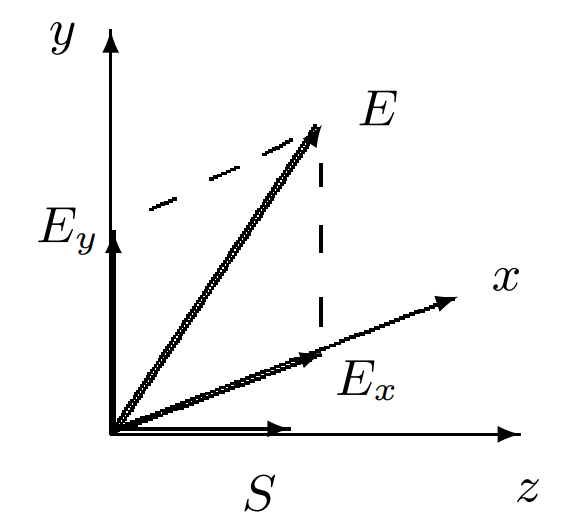
\includegraphics[width=\linewidth]{fig1}
	\caption{Представление световой волны в виде двух линейно поляризованных волн}
\end{wrapfigure}


При помощи специальных приспособлений (поляризаторов), о которых речь будет идти дальше, естественный свет может быть превращен в \textit{линейно поляризованный}. В линейно поляризованной световой волне пара векторов \textbf{E} и \textbf{H} не изменяет с течением времени своей ориентации.

Наиболее общим типом поляризации является эллиптическая поляризация. В эллиптически поляризованной световой волне конец вектора \textbf{E} (в данной точке пространства) описывает некоторый эллипс.

При теоретическом рассмотрении различных типов поляризации часто бывает удобно проектировать вектор \textbf{E} в некоторой точке пространства на два взаимно перпендикулярных направления (рис. 1). В том случае, когда исходная волна была поляризованной, $E_x$ и $E_y$ когерентны между собой и могут быть записаны в виде

\begin{equation}
\begin{gathered}
E_x = E_{x0} \cos(kz - \omega t), \\
E_y = E_{y0} \cos(kz - \omega t - \varphi),
\end{gathered}
\end{equation}

где амплитуды $E_{x0}$, $E_{y0}$, волновой вектор k,
частота $\omega$ и сдвиг фаз $\varphi$ не зависят от времени. Формулы (1) описывают монохроматический свет. Немонохроматический свет может быть представлен суммой выражений типа (1) с различными значениями частоты $\omega$.

В плоскости $z = z_0$ вектор \textbf{E} волны (1) вращается против часовой стрелки (при наблюдении навстречу волне), если 0 < $\varphi$ < $\pi$. В этом случае говорят о левой эллиптической поляризации волны. Если же $\pi$ < $\varphi$ < 2$\pi$, вращение вектора \textbf{E} происходит по часовой стрелке, и волна имеет правую эллиптическую поляризацию


\subsubsection*{Методы получения линейно поляризованного света}

Для получения линейно поляризованного света применяются специальные оптические приспособления — поляризаторы. Направление колебаний электрического вектора в волне, прошедшей через поляризатор, называется \textit{разрешенным направлением} поляризатора.

Всякий поляризатор может быть использован для исследования поляризованного света, т. е. в качестве анализатора. Интенсивность I линейно поляризованного света после прохождения через анализатор зависит от угла, образованного плоскостью колебаний с разрешенным направлением анализатора:

\begin{equation}
I = I_0 \cos^2 \alpha
\end{equation}

Соотношение (2) носит название \textit{закона Малюса}.

\subsubsection*{Пластинка чувствительного оттенка}

\begin{wrapfigure}{l}{0.35\linewidth}
	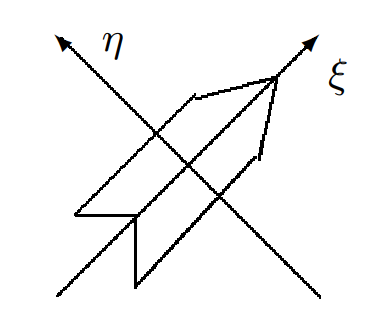
\includegraphics[width=0.8\linewidth]{fig3}
	\caption{Пластинка чувствительного оттенка}
\end{wrapfigure}

Выше предполагалось известным, какому из двух главных направлений пластинки в четверть длины волны соответствует большая скорость распространения света.
Установить это можно различными способами, например с помощью
пластинки чувствительного оттенка (так называют пластинку в $ \lambda $
для зелёной спектральной компоненты, $ \lambda = 560 $ нм).

Если пластинка чувствительного оттенка помещена между скрещенными поляроидами и главные направления пластинки не параллельны
направлениям разрешённых колебаний поляроидов, то при освещении
белым светом пластинка кажется окрашенной в лилово-красный цвет.
Это объясняется тем, что зелёная компонента линейно поляризованного света при прохождении пластинки не меняет поляризации и задерживается вторым поляроидом. Для красной и фиолетовой компонент
пластинка создаёт сдвиг фаз, несколько отличный от $ 2\pi $. На выходе
из пластинки красная и фиолетовая компоненты оказываются поэтому
эллиптически поляризованными и частично проходят через второй поляроид. Таким образом, в известном смысле наблюдаемый в указанном
опыте цвет пластинки дополнителен к зелёному.

Если между скрещенными поляроидами поместить пластинку чувствительного оттенка
($ \lambda $) и пластинку в $ \lambda/4 $ так, чтобы их главные
направления совпадали, цвет пластинки изменится. Если у пластинки чувствительного оттенка и пластинки в $ \lambda/4  $совпадут главные направления, соответствующие большей скорости распространения, то разность хода между $ E_x $ и $ E_y $ для зелёного света составит уже $ 5\lambda/4 $. Это соответствует разности хода в $ \lambda $ для света с большей длиной волны, т. е. для "<более красного"> света. При освещении
этих пластинок (напомним, что они расположены между скрещенными поляроидами) белым светом теперь погасится не зелёная, а красная
часть спектра, и проходящий свет будет казаться зеленовато-голубым.
Если же главные направления, соответствующие большей скорости распространения, у пластинки чувствительного оттенка и у пластинки
в $ \lambda/4 $ окажутся перпендикулярными, то проходящий свет приобретёт
оранжево-желтую окраску (погасится фиолетово-голубая часть спектра).

Изменение цвета позволяет, таким образом, определить, какое из
главных направлений пластинки в $ \lambda/4 $ соответствует большей скорости
распространения. 

\section*{Ход работы}

\subsubsection*{Определение разрешенных направлений поляроидов}

\begin{wrapfigure}{l}{0.3\linewidth} 
	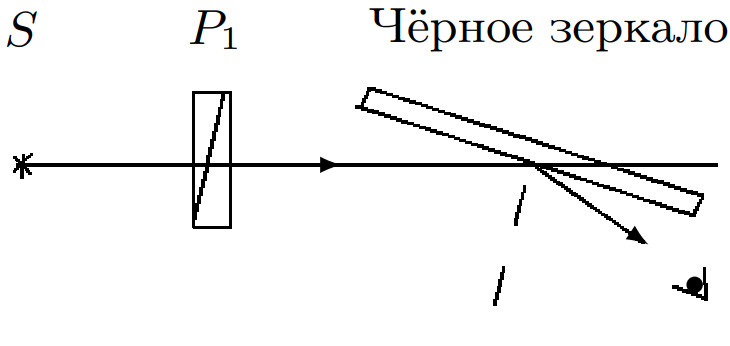
\includegraphics[width=\linewidth]{fig2}
	\caption{Определение разрешенного направления поляроида}
\end{wrapfigure}

Разместим на оптической скамье осветитель S, поляроид $P_1$ и черное зеркало. Поворачивая поляроид вокруг направления луча, добьемся наименьшей яркости пятна и, вращением зеркала вокруг вертикальной оси снова добьемся минимальной интенсивности отраженного луча. Запишем отчет по лимбу поляроида $P_1$, соответствующий найденному разрешенному направлению.

Разрешенное направление второго поляроида определим скрестив поляроиды: после поляроида с известной поляризацией поставим второй поляроид и, глядя навстречу лучу, вращением второго поляроида добьемся минимальной яркости луча. Показания лимба занесем в Таблицу 1.

\begin{table}[h!]
\begin{center}
\caption{Разрешенные направления поляризаторов}
\begin{tabular}{|c|c|c|c|c|}
\hline
   & Поляризатор 1 & Поляризатор 2  \\ \hline
  $	\alpha$, \textdegree & 348 & 35  \\ \hline
\end{tabular}
\end{center}
\end{table}
\subsubsection*{Определение угла Брюстера для эбонита}

Вместо черного зеркала поставим эбонитовую пластину.

Установим направление разрешенных колебаний поляроида $P_1$ горизонтально и найдем угол поворота эбонита $\varphi_Б$, при котором интенсивность отраженного луча минимальна. По углу поворота определим показатель преломления эбонита

\[
n = \tan(\varphi_Б) = \tan(56) \approx 1,48
\]

Повторим измерения, добавив зеленый светофильтр

\[
n = \tan(\varphi_Б) = \tan(55) \approx 1,43 
\]

\subsubsection*{Исследование стопы}

Поставим стопу стеклянных пластин вместо эбонитового зеркала и подберем для нее такое положение, при котором свет падает на стопу под углом Брюстера.

Осветим стопу неполяризованным светом и, рассматривая через поляроиды отраженный и преломленный свет определим ориентацию вектора \textbf{E}.

При наблюдении отраженного света, получили, что поляризация горизонтальная, а для преломленного света поляризация вертикальная.

\subsubsection*{Определение главных плоскостей двоякопреломляющих пластин}

Поставим кристаллическую пластинку между скрещенными поляроидами $P_1$ и $P_2$

Вращая пластинку вокруг направления луча и наблюдая за интенсивностью света, проходящего сквозь второй поляроид, определим, при каком условии главные направления пластинки совпадают с разрешёнными направлениями поляроидов. Повторите опыт для второй пластинки. Полученные данные занесем в Таблицу 2.

\begin{table}[h!]
\begin{center}
\caption{Определение главных направлений}
\begin{tabular}{|cl|cl|}
\hline
\multicolumn{2}{|c|}{пластинка   1}      & \multicolumn{2}{c|}{пластинка   2}      \\ \hline
\multicolumn{2}{|c|}{Глав напр, \textdegree} & \multicolumn{2}{c|}{Глав напр, \textdegree} \\ \hline
\multicolumn{2}{|c|}{280}                & \multicolumn{2}{c|}{222}                \\ \hline
\multicolumn{2}{|c|}{190}                & \multicolumn{2}{c|}{131}                \\ \hline
\multicolumn{2}{|c|}{100}                & \multicolumn{2}{c|}{42}                 \\ \hline
\multicolumn{2}{|c|}{10}                 & \multicolumn{2}{c|}{312}                \\ \hline
\end{tabular}
\end{center}
\end{table}

\subsubsection*{Выделение пластин $\lambda/2$ и $\lambda/4$}

Поставим между скрещенными поляроидами пластинку чувствительного оттенка ($\lambda$ для зелёного света), имеющую вид стрелки.

Уберем зелёный фильтр и поставим между скрещенными поляроидами пластинку $\lambda$ (стрелка под углом 45 \textdegree к разрешённым направлениям поляроидов). 

Добавим к схеме пластинку $\lambda / 4$, главные направления которой совпадают с главными направлениями пластинки $\lambda$ и ориентированы под углом 45 \textdegree к разрешенным направлениям скрещенных поляроидов. При повороте рейтера со стрелкой на 180 \textdegree вокруг вертикальной оси цвет стрелки меняется от зелёно-голубого до оранжево-жёлтого. 

В первом случае быстрые оси пластин совпадают, а во втором -- медленные

\subsubsection*{Интерференция поляризованных лучей}

Расположим между скрещенными поляроидами мозаичную слюдяную пластинку. 

Вращая пластинку, будем наблюдать за изменениями цвета в отдельном квадратике. В результате вращения пластинки интенсивность света, проходящего через пластинку изменяется от 0 до максимума 4 раза за один оборот.

Теперь будем вращать второй поляроид, не двигая пластинки. В результате, наблюдаем изменение цветов пластинок, причем в каких-то квадратах изменение интенсивности света происходит синфазно, а в других в противофазе. 

\begin{minipage}{.49\textwidth}
  \begin{center}
 	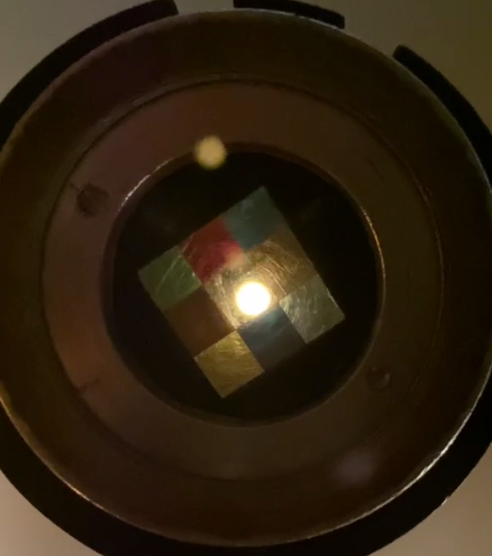
\includegraphics[width=0.6\linewidth]{fig4}
  	\captionof{figure}{}
  \end{center}
\end{minipage}
\begin{minipage}{.49\textwidth}
	\begin{center}
 		 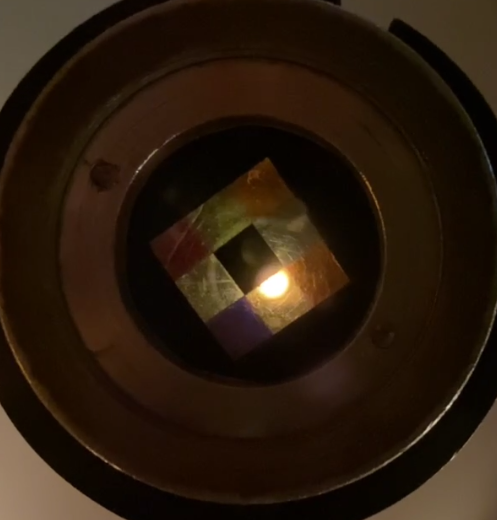
\includegraphics[width=0.6\linewidth]{fig5}
 		 \captionof{figure}{}
  	\end{center}
\end{minipage}


\section*{Выводы}
1.В результате работы мы ознакомились с методами получения и анализа поляризованного света






\end{document}
